\documentclass{beamer}
%
% Choose how your presentation looks.
%
% For more themes, color themes and font themes, see:
% http://deic.uab.es/~iblanes/beamer_gallery/index_by_theme.html
%
\mode<presentation>
{
  \usetheme{Frankfurt}
  \usecolortheme{default} % or try albatross, beaver, crane, ...
  \usefonttheme{default}  % or try serif, structurebold, ...
  \setbeamertemplate{navigation symbols}{}
  \setbeamertemplate{caption}{\raggedright\insertcaption\par}
}

\usepackage{graphicx}
\usepackage{natbib}
\usepackage[francais]{babel}
\usepackage[utf8]{inputenc}
\usepackage{amsmath}
\usepackage{amssymb}
\usepackage{mathrsfs}

\newcommand{\derivt}[1]{\frac{\partial}{\partial t} #1}
\newcommand{\derivr}[1]{\frac{\partial}{\partial r} #1}

\graphicspath{{./images/}}

\title{Simulation d'un disque d'accrétion autour d'un trou noir}
\author{Mathieu de Bony, Valentin Nourry, Sylvain Cezar,\\Jérémy Couturier, Wilfried Mercier, Thomas Nicolazo}
\date{\today}

\begin{document}

%\setbeamercolor{author}{fg=white}

{
%\usebackgroundtemplate{\includegraphics[width=\paperwidth]{images/blackhole.jpg}}%
%\setbeamercolor{background canvas}{bg=black}
\begin{frame}
  \titlepage
\end{frame}

}

% Uncomment these lines for an automatically generated outline.
%\begin{frame}{Outline}
%  \tableofcontents
%\end{frame}

\section{Introduction}

{
\usebackgroundtemplate{\includegraphics[width=\paperwidth]{Disque.jpg}}
\setbeamercolor{background canvas}{bg=black}
%\setbeamercolor{fg=white}
\begin{frame}{Introduction}
  \begin{itemize}
    \item \textcolor{white}{Binaire X}
    \item \textcolor{white}{Modélisation adaptée à des trous noirs de quelques $M_{\odot}$}
  \end{itemize}
\end{frame}
}

\section{Modélisation}

\begin{frame}{Modélisation physique}
\begin{itemize}
  \item Anneaux concentriques + orbites képlériennes
  \item $\dot{M}=\dot{M_0}$ au bord extérieur
  \item  $r_s=\frac{2GM}{c^2}$
  \item $r_{min}=3r_s$ et $r_{max}=100r_s$
  \item Composition chimique $$X=0.7,\quad Y=0.28, \quad Z=0.02$$
\end{itemize}

\end{frame}

\begin{frame}{Géométrie du disque}
    \begin{itemize}
        \item Géométrie cylindrique
        \item Modèle 1D radial
    \end{itemize}
\end{frame}

\begin{frame}{Équations}
    \begin{itemize}
        \item 13 équations : $\Omega, \mu, P, \beta, c_s, H, \rho, \nu, F_z, \dot M, v, T, \Sigma$
        \item 10 équations algébriques, 1 équation dérivée spatiale, 2 équations différentielles
    \end{itemize}
\end{frame}

\begin{frame}{Pression, indicateur de pression et masse atomique moyenne}
    \begin{itemize}
        \item $P=P_{gaz}+P_{rad}$
        \item $P_{\rm{rad}}=\frac{1}{3}aT^4$ $P_{gaz}=\frac{\rho k T}{\mu m_p}$
        \item $\mu = \frac{1}{2X+\frac{3}{4}Y+\frac{1}{2}Z}$
        \item $\beta=\frac{P_{gaz}}{P}$
    \end{itemize}
\end{frame}

\begin{frame}{Autres équations}
    \begin{itemize}
        \item $H \simeq \frac{c_s}{\Omega}$
        \item $\Omega = \Big( \frac{GM}{r^3}\Big) ^{\frac{1}{2}}$
        \item $\Sigma = 2\rho H$
        \item $\dot M = - 2 \pi r \Sigma v$
        \item $F_z=\begin{cases} \frac{2acT^4}{3(\kappa_{ff}+\kappa_e)\Sigma}, & \mbox{si } \tau_{eff} \geq 1\\ \epsilon_{ff}AH, & \mbox{si } \tau_{eff} < 1  \end{cases}$
        \item $ v = -\frac{3}{\Sigma r^{\frac{1}{2}}}\derivr{(\nu \Sigma r^{\frac{1}{2}})}$
        \item $c_s = \left ( \frac{\Gamma_1 P}{\rho} \right )^{\frac{1}{2}}$
        \item $\nu = \frac{2}{3}\alpha c_s H$
    \end{itemize}
\end{frame}

\begin{frame}{Température $T$}
    \begin{itemize}
        \item $  C_V \derivt{T}=Q^+ - Q^- +Q_{adv}$
        \item $Q^+ = \frac{9}{4}\nu \Omega ^2$
        \item $Q^-= 2\frac{F_z}{\Sigma}$
        \item $Q_{\rm{adv}} = C_V\Big[ (\Gamma_3 - 1) \frac{T}{\Sigma}\Big( \derivt{\Sigma}+v\derivr{\Sigma} \Big) -v\derivr{T} \Big]$
        \item  $C_V = \frac{R}{\mu}\frac{12(\gamma_g -1)((1-\beta)+\beta)}{(\gamma_g - 1)\beta} \text{,} \quad C_V(\Gamma_3 -1) = \frac{R}{\mu}\frac{4-3\beta}{\beta}$
    \end{itemize}
\end{frame}

\begin{frame}{Densité surfacique $\Sigma$}
    \begin{itemize}
        \item $  C_V \derivt{T}=Q^+ - Q^- +Q_{adv}$
        \item $Q^+ = \frac{9}{4}\nu \Omega ^2$
        \item $Q^-= 2\frac{F_z}{\Sigma}$
        \item $Q_{\rm{adv}} = C_V\Big[ (\Gamma_3 - 1) \frac{T}{\Sigma}\Big( \derivt{\Sigma}+v\derivr{\Sigma} \Big) -v\derivr{T} \Big]$
        \item  $C_V = \frac{R}{\mu}\frac{12(\gamma_g -1)((1-\beta)+\beta)}{(\gamma_g - 1)\beta} \text{,} \quad C_V(\Gamma_3 -1) = \frac{R}{\mu}\frac{4-3\beta}{\beta}$
        
        \item $\frac{\partial {\Sigma}}{\partial t} = \frac{3}{r}\derivr{ \big \{ r^{\frac{1}{2}} \derivr{(\nu \Sigma r^{\frac{1}{2}})} \big \}}$
    \end{itemize}
\end{frame}

\begin{frame}{Initialisation du disque}
    \begin{itemize}
        \item $T = 1,4.10^4 \alpha^{-\frac{1}{5}} \left(\frac{\dot{M}}{10^{13}\ kg.s^{-1}} \right)^{\frac{3}{10}} \left(\frac{M}{M_{\odot}} \right)^{\frac{1}{4}} \left(\frac{r}{10^8\ m} \right)^{-\frac{3}{4}} f^{\frac{3}{10}}\ K $
        \item $\Sigma = 52 \alpha^{-\frac{4}{5}} \left(\frac{\dot{M}}{10^{13}\ kg.s^{-1}} \right)^{\frac{7}{10}} \left(\frac{M}{M_{\odot}} \right)^{\frac{1}{4}} \left(\frac{r}{10^8\ m} \right)^{-\frac{3}{4}} f^{\frac{7}{10}}\ kg.cm^{-2}$
    \end{itemize}
    \begin{figure}
        \includegraphics[width = 0.48\linewidth]{ProfileRtemperatureInit.pdf}
        \includegraphics[width = 0.48\linewidth]{ProfileRsigmaInit.pdf}
    \end{figure}    
\end{frame}

\section{L'adimensionnement}

\begin{frame}{Adimensionnement}
\begin{itemize}
	\item Valeurs numériques en SI très grandes
	\item Puissance de ces grandes valeurs
	\item L'adimensionnement permet de se rapprocher de l'unité
	\item $[X]=kg^{\alpha}m^{\beta}s^{\gamma}K^{\delta}$
	\item Quatres constantes fondamentales
	\begin{align}
		[r_s]=kg^{0}m^{1}s^{0}K^{0}\\
		[\Omega_{\rm{max}}]=kg^{0}m^{0}s^{-1}K^{0}\\
		[\dot{M_0}]=kg^{1}m^{0}s^{-1}K^{0}\\
		[\mathcal{R}]=kg^{0}m^{2}s^{-2}K^{-1}
	\end{align}
	\begin{equation}
	  X\;\;\textrm{où}\;\;[X]=kg^{\alpha}m^{\beta}s^{\gamma}K^{\delta} \rightarrow r_s^{2\delta+\beta}\;\Omega_{\rm{max}}^{2\delta-\gamma-\alpha}\;\dot{M_0}^{\alpha}\;\mathcal{R}^{-\delta}\;X
	\end{equation}
\end{itemize}
\end{frame}

\begin{frame}{Adimensionnement}
	\begin{equation}
		F_z=\frac{2acT^4}{3(\kappa_{ff}+\kappa_e)\Sigma}\rightarrow F_z=\frac{acr_s^8\Omega_{max}^6}{\mathcal{R}^4\dot{M}_0}\frac{xT^4}{(\kappa_{ff}+\kappa_e)S}
	\end{equation}
	\begin{itemize}
	  \item Certaines équations sont trop compliquées $\rightarrow$ Plus d'erreurs
	  \item On ne s'éloigne pas de l'unité
	\end{itemize}
	Essaie d'une nouvelle méthode d'adimensionnement
\end{frame}

\begin{frame}{Deuxième méthode}
\begin{itemize}
  \item Autant de constantes que de grandeurs que la simulation fait intervenir.
  \item Les constantes deviennent $1$.
  \item Toutes les équations sont simplifiées.
\end{itemize}
	\begin{equation}
		F_z=\frac{2acT^4}{3(\kappa_{ff}+\kappa_e)\Sigma}\rightarrow F_z=\frac{xT^4}{3(\kappa_{ff}+\kappa_e)S}
	\end{equation}
\end{frame}

\begin{frame}{Théorème de Vaschy-Buckingham}
  \begin{itemize}
  \item Le problème fait intervenir 13 inconnus $\Omega,\mu,P,\beta,c_s,H,\rho,\nu,\Sigma,v,\dot{M},T\;\textrm{et}\;F_z$.
  \item Il existe une fonction $f$ telle que $f(\Omega,\mu,P,\beta,c_s,H,\rho,\nu,\Sigma,v,\dot{M},T,F_z)=0$
  \item Seules $4$ de ces grandeurs sont dimensionnellement indépendantes.
  \end{itemize}
  On adimensionne avec :
  \begin{align}
  [T]=K\\
  [\rho v^2]=kg.m^{-1}.s^{-2}\\
  [v]=m.s^{-1}\\
  [H]=m
  \end{align}
\end{frame}

\begin{frame}{Vaschy-Buckingham}
  Il existe $g$ telle que :
  \begin{equation}
    g(\mu,\beta,\frac{\Omega H}{v},E_u,M_a,\mathcal{R}_e,\frac{\Sigma}{\rho H},\frac{\dot{M}}{\rho vH^2},\frac{F_z}{\rho v^3})=0
  \end{equation}
  Avec :
  \begin{align}
    E_u=\frac{P}{\rho v^2}\\
    M_a=\frac{v}{c_s}\\
    \mathcal{R}_e=\frac{Hv}{\nu}
  \end{align}
  Or: $\frac{\Omega H}{v}=\frac{1}{M_a}$, $\frac{\Sigma}{\rho H}=2$.
  On peut se ramener à 7 variables.
\end{frame}

\section{Équations différentielles}

\begin{frame}{Les échelles de temps}

Équation d'évolution de la densité de surface
\begin{equation}
    \frac{\partial {\Sigma}}{\partial t} = \frac{3}{r}\frac{\partial}{\partial r}\left[\sqrt{r}\frac{\partial}{\partial r}(\nu \Sigma\sqrt{r})\right]
    \end{equation}
\begin{block}{Temps visqueux}
\[
 t_\text{visc} = \frac{r^2}{\nu}
\]
\end{block}

Équation d'évolution de la température
\begin{equation}
    C_V \frac{\partial T}{\partial t}=Q^+ - Q^- +Q_{adv}
\end{equation}
\begin{block}{Temps thermique}
\[
t_\text{th} = t_\text{visc} \left(\frac{H}{r}\right)^2
\]
\end{block}
\end{frame}

\begin{frame}{Les échelles de temps}
\begin{block}{Comparaison  des temps caractéristiques}
\[
t_\text{th} \approx t_\text{dyn} \ll t_\text{visc}\text{  , avec   } t_\text{dyn} = \frac{1}{\Omega}
\]
\end{block}

Réunion de processus physiques très rapides et très lents les uns par rapport aux autres.

\pause

$\Rightarrow $  Comment implémenter des échelles de temps différents de plusieurs ordres de grandeur dans la même simulation ?

\end{frame}

\begin{frame}{Schémas d'Euler}
\begin{equation}
    \frac{\partial {\Sigma}}{\partial t} = \frac{3}{r}\frac{\partial}{\partial r}\left[\sqrt{r}\frac{\partial}{\partial r}(\nu \Sigma\sqrt{r})\right]
    \end{equation}
\begin{itemize}
\item{Explicite}
\[\Sigma^{n+1} = M\Sigma^n\]
\end{itemize}
Les grandeurs s'expriment au temps $t$, la dérivée temporelle nous permet de sortir un $\Sigma(t+\Delta t)$

$\Rightarrow$ Simple à mettre en œuvre

Mais ce schéma n'est stable que pour $ \Delta t < 2 \Delta x ^2$

\begin{itemize}
\item{Implicite}
\[\Sigma^{n} = M\Sigma^{n+1}\]
\end{itemize}

\end{frame}


\begin{frame}{Les conditions aux bords}
%\includegraphics[width = 0.6\linewidth]{schema-disque.pdf}
\begin{itemize}
\item Au bord interne
\begin{align}
S(x_\text{min}) &= 0
\end{align}
\item Au bord externe
\begin{align}
\left.3\pi\frac{\partial}{\partial x}\left(\nu S\right)\right|_{x\text{max}} &= \dot{M_0}\label{S_conditionExt}
\end{align}

\end{itemize}
\end{frame}





\section{Courbe en S}

\begin{frame}{Caractéristiques de la courbe en S}
    \begin{figure}
        \centering
        \includegraphics[width=\linewidth]{Space_pos_neg.png}
        \label{Fig:Sneg}
    \end{figure}

    \begin{block}{Equation de la courbe en S}
      \begin{equation*}
        \partial_t T \propto \delta Q (S, T) = Q^{+} - Q^{-} = 0
      \end{equation*}
    \end{block}
\end{frame}

\begin{frame}{Dichotomie}
    Deux méthodes:
    \begin{itemize}
        \item par incrément
        \setlength{\itemindent}{2em}
        \item[$\rightarrow$] détection branche du bas
        \setlength{\itemindent}{0em}
        \item par encadrement
        \setlength{\itemindent}{2em}
        \item[$\rightarrow$] toutes les solutions
    \end{itemize}
\end{frame}

\begin{frame}{Tests préliminaires}
    \begin{figure}
        \centering
        \includegraphics[width=0.49\linewidth]{Circle_dicho.png}%
        \includegraphics[width=0.49\linewidth]{DiffSquares_dicho.png}
        \caption{Résultats de la dichotomie pour $F(x,y) = X^2 +  Y^2 + \rm{cte}$ à gauche et $F(X,Y) = X^2 - Y^2$ à droite.}
        \label{Circle_dicho.png}
    \end{figure}
\end{frame}

\begin{frame}{Solution par méthode d'incréments}
    \begin{figure}[ht]
      \begin{minipage}[ht]{0.48\linewidth}
        \centering
        \includegraphics[width=\textwidth]{Nice_S_curve}
        \caption{Solution trouvée par notre code.}
        $\rightarrow$ Mauvaise branche du haut détectée !
      \end{minipage}
      \hspace{5pt}
      \begin{minipage}[ht]{0.4\linewidth}
        \centering
        \includegraphics[width=\textwidth]{LasotaScurve2.png}
        \caption{Solution de Lasota et al.}
      \end{minipage}
    \end{figure}
\end{frame}

\begin{frame}{Branche du haut physique et discontinuité}
  \begin{columns}
    \column{0.58\linewidth}
      \includegraphics[width=\textwidth]{3D_discontinuity_magnified.png}

    \column{0.42\linewidth}
      Lasota et al. :
      \begin{itemize}
        \item "One notices immediately that the upper branch coincides with the $\tau_{\rm{eff}} = 1$ line."
        \item "After reaching this point the system oscillates along an upper equilibrium branch."
      \end{itemize}
  \end{columns}
\end{frame}

\begin{frame}{Branche physique du haut et discontinuité}
  \begin{columns}
    \column{0.58\linewidth}
      \includegraphics[width=0.8\textwidth]{Lasotaetal.png}

    \column{0.42\linewidth}
      Lasota et al. :
      \begin{itemize}
        \item "One notices immediately that the upper branch coincides with the $\tau_{\rm{eff}} = 1$ line."
        \item "After reaching this point the system oscillates along an upper equilibrium branch."
      \end{itemize}
  \end{columns}
\end{frame}

\subsection{Mesh en température et densité}

\begin{frame}{Principe}
	\begin{minipage}[c]{.46\linewidth}
      \includegraphics[width = 0.95\linewidth]{DecoupeR}
   \end{minipage} \hfill
   \begin{minipage}[c]{.46\linewidth}
      \includegraphics[width = 0.95\linewidth]{SPrincipe}
   \end{minipage}
\end{frame}

\begin{frame}{Implémentation du mesh}
\begin{itemize}
	\item Choix du range exploré en température et en densité
	\item Création du set de coordonnées en fonctions des bornes et du nombre d'échantillon
	\item Calcul pour chaque paire possible de coordonnées des termes de chauffage et de refroidissement
	\item Calcul des encadrements
	\item Sortie dans un fichier ou utilisation de données pour guider la dichotomie
\end{itemize}
\end{frame}

\begin{frame}{Mesh obtenu}
	\centering Courbe en S à une distance de $14.4 R_s$ pour un trou noir de $10 M_{\odot}$
	\begin{minipage}[c]{.49\linewidth}
      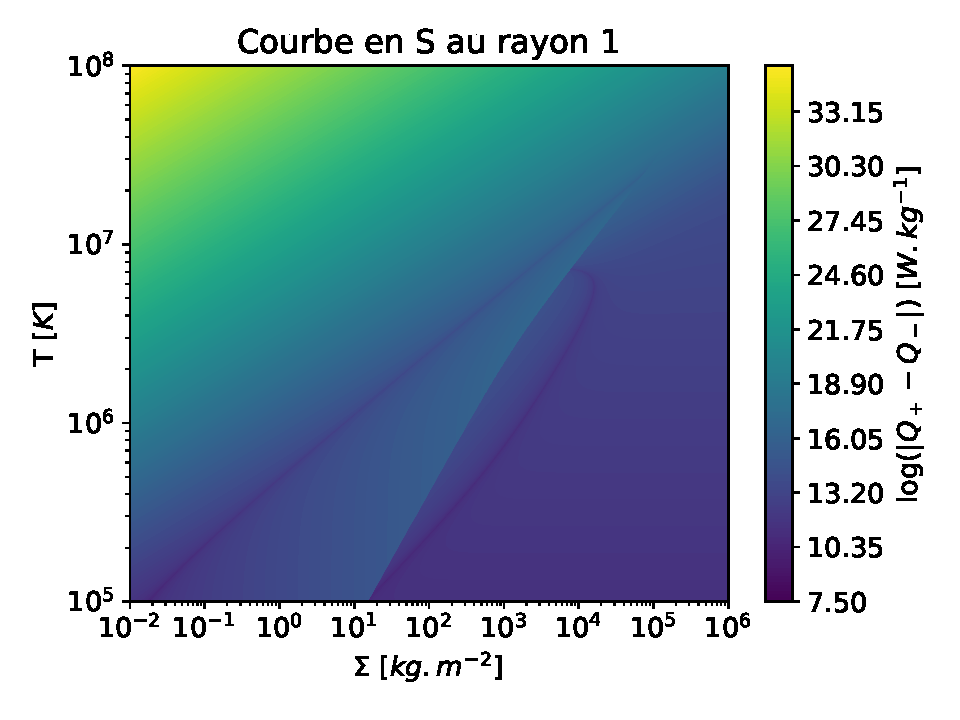
\includegraphics[width = 0.98\linewidth]{SLog-1}
   \end{minipage} \hfill
   \pause
   \begin{minipage}[c]{.49\linewidth}
      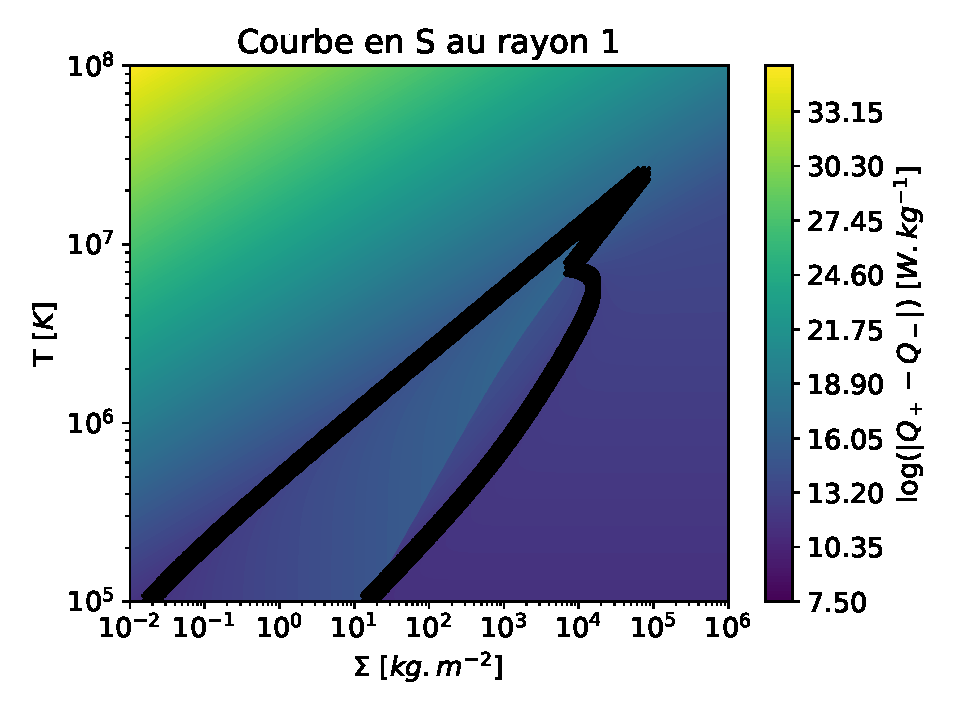
\includegraphics[width = 0.98\linewidth]{SLogFrame-1}
   \end{minipage}
\end{frame}

\begin{frame}{Mesh obtenu}
	\centering Courbe en S à une distance de $14.4 R_s$ et 100 $R_s$\\ pour un trou noir de $10 M_{\odot}$
	\\
	\begin{minipage}[c]{.49\linewidth}
      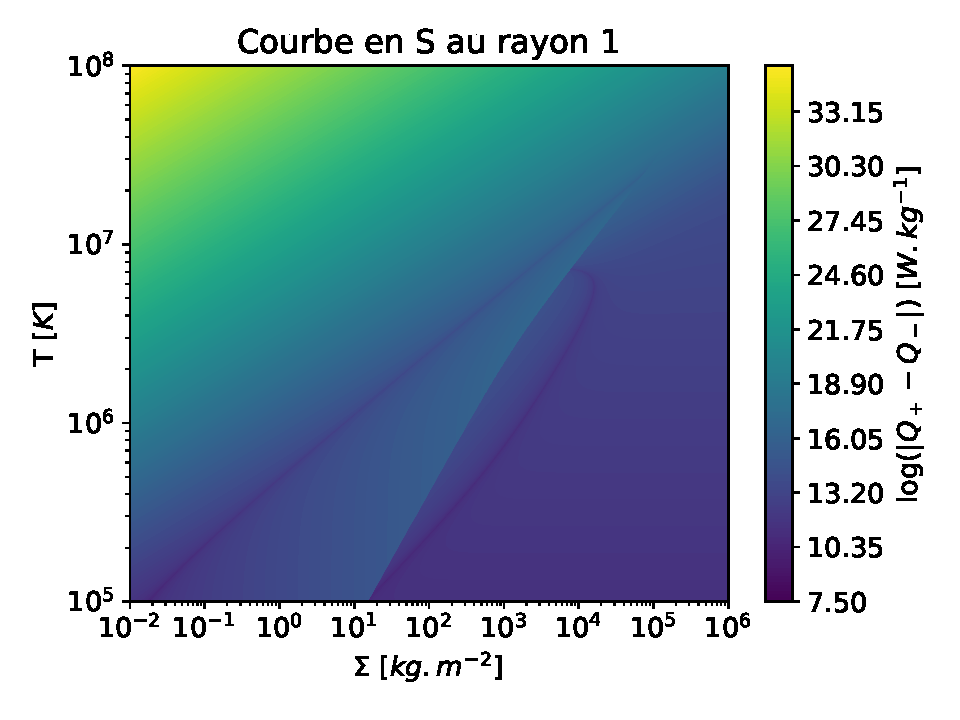
\includegraphics[width = 0.98\linewidth]{SLog-1}
   \end{minipage} \hfill
   \begin{minipage}[c]{.49\linewidth}
      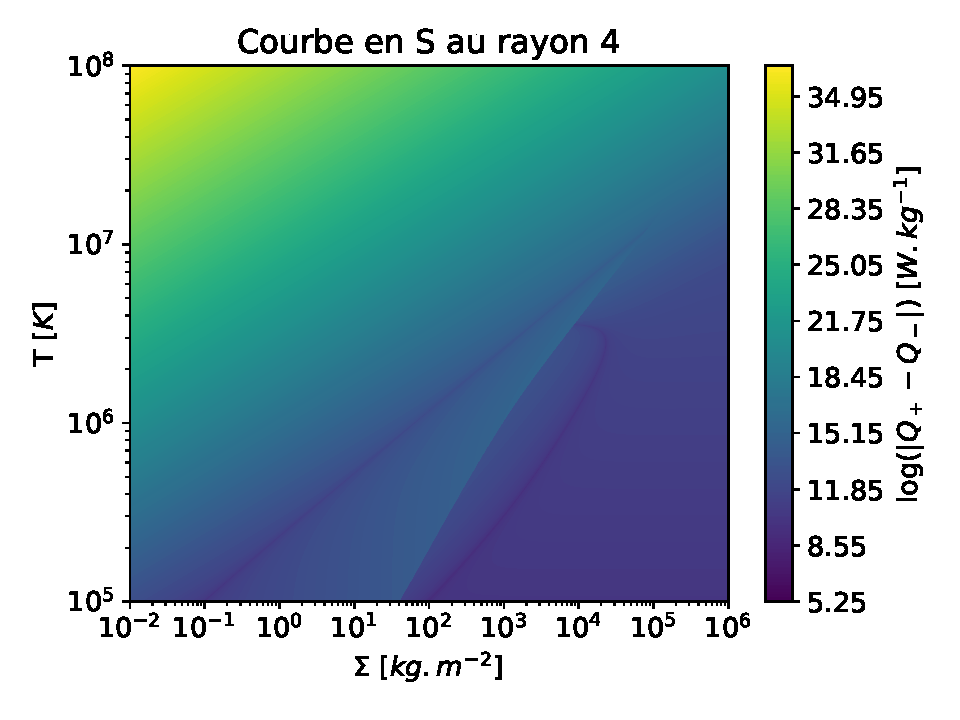
\includegraphics[width = 0.98\linewidth]{SLog-4}
   \end{minipage}
\end{frame}



\begin{frame}{Structure du code}

\includegraphics[width = 1.0\linewidth]{images/structure.pdf}

Et des codes python pour afficher les résultats.
\end{frame}



\section{Résultats et discussion}
\begin{frame}{Évolution du disque}
	\centering
	Évolution du taux d'accrétion dans un disque \\avec un taux d'accrétion extérieur de $5.10^{13} kg.s^{-1}$ \\autour d'un trou noir de $10 M_{\odot}$\\
	\includegraphics[width = 0.7\linewidth]{accretionRate10M}
\end{frame}

\begin{frame}{Évolution du disque}
	\centering
   \begin{minipage}[c]{.49\linewidth}
      \includegraphics[width = 0.98\linewidth]{accretionRate10M}
   \end{minipage} \hfill
   \begin{minipage}[c]{.49\linewidth}
      \includegraphics[width = 0.98\linewidth]{accretionRate-stable}
   \end{minipage}
\end{frame}

\begin{frame}{Évolution du disque sur la courbe en S}
 \centering
 Évolution sur la courbe en S à un distance de $50.4 R_s$ \\avec un trou noir de $10 M_{\odot}$
 \includegraphics[width=0.8\linewidth]{SLog-130}
\end{frame}

\begin{frame}{Évolution du disque en fonction de la masse du trou noir}
	\centering
	Évolution du taux d'accrétion \\pour un trou noir de $5 M_{\odot}$, $10 M_{\odot}$ et $15 M_{\odot}$
   \begin{minipage}[c]{.49\linewidth}
      \includegraphics[width = 0.85\linewidth]{accretionRate5M}
   \end{minipage} \hfill
   \begin{minipage}[c]{.49\linewidth}
      \includegraphics[width = 0.85\linewidth]{accretionRate10M}
   \end{minipage}
   \includegraphics[width = 0.44\linewidth]{accretionRate15M}
\end{frame}

\begin{frame}{Forme du disque}
	\centering
   \begin{minipage}[c]{.49\linewidth}
      \includegraphics[width = 0.85\linewidth]{ProfileRsigma}
   \end{minipage} \hfill
   \begin{minipage}[c]{.49\linewidth}
      \includegraphics[width = 0.85\linewidth]{ProfileRtemperature}
   \end{minipage}
   \pause
   \includegraphics[width = 0.44\linewidth]{ProfileRheight}
\end{frame}


\section{Conclusion}
\begin{frame}{Outils numériques et compétences}
\begin{itemize}
\item Fortran 90
\item Make, Makefile
\item Introduction à l'outil Git
\item Écriture d'outils numériques et utilisation de Lapack
\item Écriture d'outils d'analyse en python
\item rédaction \LaTeX
\end{itemize}
\end{frame}


\begin{frame}{Perspectives}
\begin{itemize}
\item Transition optique de optiquement épais à optiquement mince
\item Meilleure sélection entre les pas de temps visqueux et thermiques
\item Étude du disque dans les zones instables, et au point critique
\end{itemize}

\end{frame}



\section{Contenu additionnel}
  \begin{frame}{Courbes en S}
    \centering
    \includegraphics[width=0.7\linewidth]{3D_SCurves_magnified.png}
  \end{frame}

  \begin{frame}{Courbes en S}
    \centering
    \includegraphics[width=0.7\linewidth]{2D_SCurvespng.png}
  \end{frame}

  \begin{frame}{Zoom sur la discontinuité}
    \centering
    \includegraphics[width=0.7\linewidth]{2D_discontinuity.png}
  \end{frame}

  \begin{frame}{Opacité autour de la courbe en S}
    \centering
    \includegraphics[width=0.7\linewidth]{TAUEFF_equiv.png}
  \end{frame}
  
  \begin{frame}{Points de pente maximale}
    \centering
        \includegraphics[width=0.7\linewidth]{MaxSlopePoint.png}
  \end{frame}



\end{document}
